\chapter{Grundlagen}
\label{chap:grundlagen}

Dieses Kapitel erarbeitet die fachlichen Grundlagen der Arbeit. Abschnitt~\ref{sec:cyber-ranges}
führt in Cyber Ranges ein, ordnet den Begriff ein und grenzt ihn von verwandten Konzepten ab.
Abschnitt~\ref{sec:cyber-resilienz} behandelt Cyber-Resilienz als konzeptionellen Rahmen, und
Abschnitt~\ref{sec:vuln-scanner} legt die Grundlagen zu Schwachstellen-Scannern, die im ersten
Use Case verglichen werden.

\section{Cyber Ranges}
\label{sec:cyber-ranges}

\subsection{Begriff und Abgrenzung}
\label{subsec:cr-begriff}

Cyber Ranges werden als komplexe, virtuelle Umgebungen beschrieben, die reale
Cybersecurity-Situationen -- etwa Angriffe oder Cyberwarfare -- nachbilden und in einem
kontrollierten Rahmen sowohl praxisnahes Training als auch Forschung und die Untersuchung
unterschiedlicher Szenarien ermöglichen \cite[2--3]{IntroductionCyberRanges2022}. Als kennzeichnend
gilt dabei die Kombination aus realitätsnaher Simulation, einer virtuellen Umgebung, in der
mehrere Teams agieren können, sowie einer leistungsbasierten Bewertung der durchgeführten
Übungen \cite[2--3]{IntroductionCyberRanges2022}. In der wissenschaftlichen Literatur werden Cyber
Ranges übereinstimmend als virtuelle, isolierte IT-Landschaften charakterisiert, in denen sich
sicherheitsrelevante Ereignisse analysieren lassen, ohne produktive Systeme zu gefährden
\cite{Chouliaras2021}.

Von klassischen \emph{Testbeds} unterscheiden sich Cyber Ranges weniger durch die zugrunde
liegende technische Infrastruktur als vielmehr durch ihren szenarienorientierten Charakter.
Während Testbeds primär auf die Untersuchung einzelner Technologien oder Netzwerkkonfigurationen
ausgerichtet sind, kombinieren Cyber Ranges Infrastruktur, Benutzerinteraktion und zeitliche
Abläufe innerhalb eines integrierten Szenariokonzepts und eignen sich dadurch für die
Untersuchung komplexer, mehrstufiger Sicherheitsereignisse \cite[2]{Chouliaras2021}. Ähnlich
adressieren \emph{Digital Twins} und Testbeds auf Systemebene typischerweise die Abbildung und
Validierung eines konkreten Systems, während Cyber Ranges primär der reproduzierbaren
Bereitstellung variabler Übungs- und Experimentierumgebungen für Angriffs-, Verteidigungs- und
Evaluationsszenarien dienen.

Ursprünglich wurden Cyber Ranges vor allem für Ausbildungs- und Trainingszwecke entwickelt. In
der Literatur wird jedoch zunehmend ihre Nutzung als Forschungsumgebung hervorgehoben,
insbesondere dann, wenn reproduzierbare Szenarien und strukturierte Bewertungsmechanismen
vorgesehen sind: Durch die kontrollierte, wiederholbare Durchführung identischer Szenarien lassen
sich unterschiedliche Werkzeuge, Strategien oder Vorgehensweisen unter vergleichbaren Bedingungen
untersuchen \cite[2]{Chouliaras2021,Yamin2020CyberRanges}. Ein wesentliches Merkmal moderner
Cyber Ranges ist damit die Verbindung von Lern-, Trainings- und Validierungsaspekten innerhalb
einer gemeinsamen Umgebung \cite{IntroductionCyberRanges2022}.

Für die vorliegende Arbeit ist insbesondere diese forschungsorientierte Perspektive relevant.
Während Trainings- und Testaspekte als notwendige Bestandteile moderner Cyber Ranges betrachtet
werden, liegt der Schwerpunkt hier auf der Nutzung einer Cyber Range als \emph{reproduzierbare
Forschungsumgebung}. Diese Einordnung bildet die begriffliche Grundlage für die weiteren
Abschnitte und für die spätere Ableitung von Anforderungen an die Plattformauswahl.

\subsection{Architektur und Komponenten}
\label{subsec:cr-architektur}

Die konkrete Architektur einer Cyber Range hängt von ihrem Einsatzzweck ab: Eine Plattform
kann sämtliche Funktionen abdecken oder gezielt auf eine Spezialisierung -- etwa Forschung,
Security-Testing ausgerichtet sein \cite[13]{IntroductionCyberRanges2022}.
Übergreifend lässt sich jedoch ein verbreitetes Architekturmodell beschreiben, das aus fünf
funktionalen Modulen besteht \cite[13]{IntroductionCyberRanges2022}:

\begin{itemize}
  \item \textbf{Portal:} stellt die Benutzeroberfläche und die Zugangsschicht bereit; der
        Zugriff auf virtuelle bzw.\ cloud-basierte Cyber Ranges erfolgt typischerweise über
        einen Webbrowser und einen Webserver (z.\,B.\ Nginx oder Apache).
  \item \textbf{Laufzeitumgebung:} führt die Szenarien aus und unterstützt simulationsbasierte Umgebungen sowie die Erzeugung von Netzwerkverkehr zur realitätsnahen
        Nachbildung.
  \item \textbf{Management:} betrifft die Ressourcenzuteilung sowie Team- und Aufgabenverwaltung
        während der Durchführung einer CSE (Cyber Security Exercise).
  \item \textbf{Datenbank:} speichert Übungsmodule, Statistiken und Logs. Eingesetzt werden dabei 
        relationale (MySQL) oder NoSQL-Datenbanken.
  \item \textbf{Monitoring:} erfasst und überwacht den Ablauf der Übungen sowie Mess- und
        Auswertungsdaten für Forschung und Produkttests.
\end{itemize}

Die Laufzeitumgebung stützt sich dabei auf unterschiedliche Werkzeugklassen: Virtualisierungswerkzeuge (z.\,B.\ VMware, VirtualBox, KVM oder QEMU sowie Cloud-Frameworks wie
OpenNebula) bilden Systeme als virtuelle Maschinen ab, Simulationswerkzeuge modellieren das
Verhalten ganzer Netze, und Traffic-Generatoren erzeugen realistischen Datenverkehr
\cite[14--21]{IntroductionCyberRanges2022}. In der Forschungsliteratur wird die Architektur entsprechend
als eine der zentralen Dimensionen zur Charakterisierung von Cyber Ranges geführt -- neben
Szenarien, Funktionen und Werkzeugen \cite{Yamin2020CyberRanges}.

Die in dieser Arbeit eingesetzte Plattform setzt dieses Modell konkret um: Ein Web-Portal bildet
die Zugangsschicht, die Bereitstellung der Szenarien (Sandboxes) erfolgt automatisiert auf einer
virtualisierten Cloud-Infrastruktur, und die Lebenszyklusverwaltung übernehmen dedizierte
Management-Dienste. Diese Umsetzung wird in Kapitel~\ref{chap:stand-der-technik} sowie bei der
Implementierung der Forschungsumgebung gezeigt.

\subsection{Typen von Cyber Ranges}
\label{subsec:cr-typen}

Nach Art der technischen Realisierung lassen sich Cyber Ranges in drei Typen einteilen --
physisch, virtuell und hybrid (Abbildung~\ref{fig:cr-typen})
\cite[47--63]{IntroductionCyberRanges2022}.

\begin{figure}[H]
  \centering
  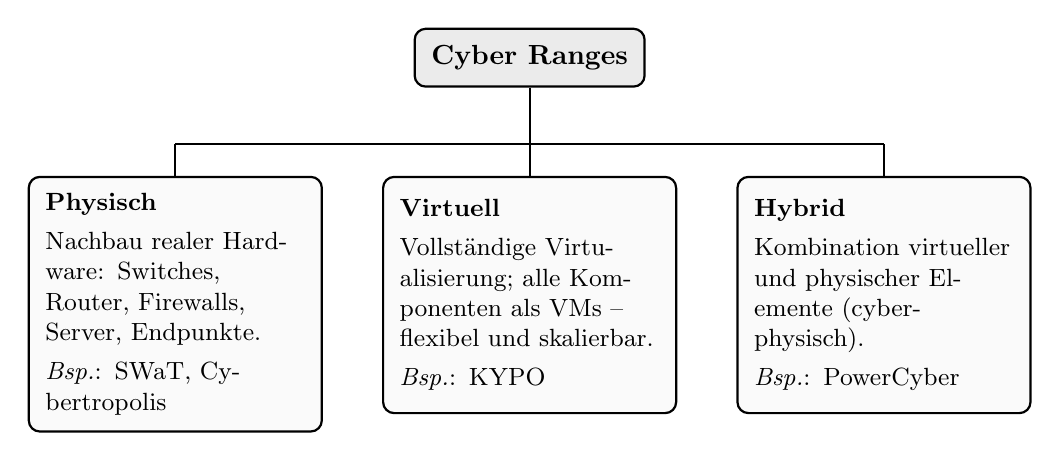
\begin{tikzpicture}[
      font=\small,
      box/.style={
        draw, rounded corners, thick, fill=black!2,
        text width=3.3cm, align=left, inner sep=6pt,
        minimum height=3cm, anchor=north
      },
      root/.style={
        draw, rounded corners, thick, fill=black!8,
        inner sep=6pt, font=\bfseries
      }
    ]
    \node[root] (root) at (0,0) {Cyber Ranges};

    \node[box] (phys) at (-4.5,-1.5) {\textbf{Physisch}\\[3pt]
      Nachbau realer Hardware: Switches, Router, Firewalls, Server,
      Endpunkte.\\[3pt]
      \emph{Bsp.}: SWaT, Cybertropolis};
    \node[box] (virt) at (0,-1.5) {\textbf{Virtuell}\\[3pt]
      Vollständige Virtualisierung; alle Komponenten als VMs -- flexibel
      und skalierbar.\\[3pt]
      \emph{Bsp.}: KYPO};
    \node[box] (hybr) at (4.5,-1.5) {\textbf{Hybrid}\\[3pt]
      Kombination virtueller und physischer Elemente (cyber-physisch).\\[3pt]
      \emph{Bsp.}: PowerCyber};

    \draw[thick] (root.south) -- (0,-1.1);
    \draw[thick] (-4.5,-1.1) -- (4.5,-1.1);
    \draw[thick] (-4.5,-1.1) -- (phys.north);
    \draw[thick] (0,-1.1) -- (virt.north);
    \draw[thick] (4.5,-1.1) -- (hybr.north);
  \end{tikzpicture}
  \caption{Typen von Cyber Ranges (eigene Darstellung in Anlehnung an \cite{IntroductionCyberRanges2022})}
  \label{fig:cr-typen}
\end{figure}

Eine physische Cyber Range bildet die reale Infrastruktur vollständig nach. Komponenten
wie Firewalls, Server und Router werden als echte Hardware dupliziert. Das wirkt sehr realistisch, ist jedoch mit erheblichen Nachteilen verbunden -- hohe Anschaffungs- und
Betriebskosten, großer Strom- und Kühlbedarf sowie aufwändige Auf- und Rückbauprozesse
\cite[54]{IntroductionCyberRanges2022}. Typische Beispiele sind SCADA-Testbeds wie SWaT und WADI
oder die frühe USMA~IWAR.

Eine virtuelle Cyber Range besteht vollständig aus virtualisierten Komponenten, die als
virtuelle Maschinen abgebildet werden. Gegenüber physischen Umgebungen sinken Kosten und Aufwand
deutlich: Umgebungen lassen sich bei Bedarf schnell bereitstellen, nach einer Übung zurücksetzen,
flexibel skalieren und auf handelsüblicher Hardware betreiben \cite[60]{IntroductionCyberRanges2022}.
Als Einschränkung gilt, dass sich nicht jedes Szenario realitätsgetreu nachbilden lässt -- die
exakte Modellierung physischer Komponenten ist im virtuellen Umfeld schwieriger. 

Eine hybride Cyber Range kombiniert virtuelle und physische Elemente (cyber-physische
Range) und vereint so die Skalierbarkeit virtueller Umgebungen mit dem Realismus physischer
Komponenten. Der Anteil beider richtet sich nach den Anforderungen des Szenarios
\cite[47]{IntroductionCyberRanges2022}. Beispiele sind EVA, DIATEAM und CRATE.

Unabhängig vom Typ wird zwischen Betriebsmodellen unterschieden: Bei einer On-Premise-Cyber
Range betreibt die Organisation die Plattform selbst, was maximale Kontrolle ermöglicht, aber
kostenintensiver ist. Cyber Range as a Service(CRaaS) wird hingegen cloudbasiert von einem
Anbieter bereitgestellt und ist schnell und wirtschaftlich verfügbar, geht jedoch mit geringerer
Kontrolle über die Infrastruktur einher \cite[63]{IntroductionCyberRanges2022}. Die vorliegende
Arbeit setzt auf eine virtuelle, selbst betriebene (On-Premise) Cyber Range, da die
Reproduzierbarkeit, Kostenkontrolle und Skalierbarkeit für eine Forschungsumgebung am wichtigsten sind. 

\subsection{Einsatzzwecke: Testing, Training und Forschung}
\label{subsec:cr-einsatzzwecke}

Cyber Ranges werden für drei übergeordnete Einsatzzwecke genutzt -- Testing, Training und
Forschung. Diese unterscheiden sich aber weniger durch die zugrunde liegende Technik als durch Zielsetzung,
Szenariogestaltung und Art der Ergebnisbewertung \cite[67]{IntroductionCyberRanges2022}\cite{Chouliaras2021}.

Im Testing dienen Cyber Ranges der Überprüfung von Systemen, Softwarekomponenten und
Sicherheitsmechanismen. Typische Verfahren sind Penetration-, Software- und Security-Testing \cite[67--72]{IntroductionCyberRanges2022}. 

Im Training steht der Aufbau von Kompetenz im Umgang mit Sicherheitsvorfällen im
Vordergrund -- wie etwa Awareness-Schulungen und Incident-Response-Übungen, in denen Teams unter
realitätsnahen Bedingungen Erkennung, Analyse und Reaktion üben \cite[72]{IntroductionCyberRanges2022}.

Im Forschungskontext werden Cyber Ranges als experimentelle Umgebungen zum systematischen
Erkenntnisgewinn genutzt, um Werkzeuge zu vergleichen oder das Verhalten von Systemen unter
definierten Bedingungen zu analysieren. Zentrale Anforderungen sind dabei Nachvollziehbarkeit und
Reproduzierbarkeit der Szenarien, sodass Ergebnisse nicht nur situationsbezogen interpretiert,
sondern verallgemeinert werden können \cite[76--78]{IntroductionCyberRanges2022}\cite{Chouliaras2021,Yamin2020CyberRanges}.

\section{Cyber-Resilienz}
\label{sec:cyber-resilienz}

\subsection{Begriff und Einordnung}
\label{subsec:resilienz-begriff}

Klassische Sicherheitsansätze zielen vor allem auf Vermeidung und Schutz ab. Cyber-Resilienz geht
einen Schritt weiter. Sie beschreibt die Fähigkeit eines Systems, auch unter Störungen oder
Angriffen zentrale Funktionen aufrechtzuerhalten und sich nach einem Ereignis wieder zu
stabilisieren. NIST fasst das in vier Fähigkeiten zusammen: widrige Bedingungen und Angriffe zu
antizipieren, zu überstehen, sich davon zu erholen und sich daran anzupassen (anticipate,
withstand, recover, adapt) \cite{NISTSP800160v2}.

Linkov et al. liefern dazu einen metrikenorientierten Ansatz. Sie verstehen Resilienz als
dynamische Eigenschaft eines Systems, die sich über mehrere Phasen eines Ereignisses beschreiben
und bewerten lässt \cite[2--3]{Linkov2013ResilienceMetrics}. Resilienz ist also kein fester Zustand
von sicher oder unsicher. Sie zeigt sich vielmehr im Verlauf der Systemleistung über die Zeit, von
einem Einbruch über die Wiederherstellung bis zur Anpassung \cite[3--5]{Linkov2013ResilienceMetrics}.

\subsection{Modelle und Metriken}
\label{subsec:resilienz-modelle}

Als Rahmen führen Linkov et al. eine Resilience-Matrix ein. Sie verbindet vier Fähigkeiten eines
Systems (plan/prepare, absorb, recover, adapt) mit verschiedenen Systemdomänen. Dadurch wird
Cyber-Resilienz mess- und vergleichbar. Kennzahlen erfassen dann nicht nur die Prävention, sondern
auch die Robustheit im Ereignisfall, die Wiederherstellung und die Anpassung
\cite[3--4]{Linkov2013ResilienceMetrics}. Diese vier Phasen decken sich weitgehend mit den
Resilienzzielen von NIST. Zusammen beschreiben sie den Lebenszyklus eines Sicherheitsereignisses
über die Zeit \cite{NISTSP800160v2}.

Neuere Arbeiten setzen den Schwerpunkt stärker auf eine missionsorientierte Sicht. Xiong et al.
schlagen dazu das Mission-Oriented Security Framework (MOSF) vor. Es verankert Cyber-Resilienz als
Gestaltungsziel und richtet Sicherheitsmaßnahmen an der Mission des Systems aus
\cite{Xiong2023MissionOrientedResilience}. Ein vollständig verwundbarkeitsfreies System wird dabei
nicht vorausgesetzt. Stattdessen soll das System seine Ziele auch unter Angriffen und Fehlern in
ausreichender Qualität erreichen \cite{Xiong2023MissionOrientedResilience}.

\subsection{Bezug zu dieser Arbeit}
\label{subsec:resilienz-bezug}

Diese phasenorientierte Sicht ist für diese Arbeit wichtig. Sie verbindet das Konzept der Resilienz
mit konkreten Werkzeugen. Die Schwachstellen-Scanner aus dem ersten Use Case gehören in die
vorbereitende Phase. Das ist der plan/prepare-Schritt bei Linkov und das Anticipate-Ziel bei NIST.
Solche Scanner finden Schwachstellen und Fehlkonfigurationen, bevor ein Angriff passiert. Damit
stärken sie die Vorbereitung eines Systems.

Wie gut diese Vorbereitung ist, beeinflusst direkt die späteren Phasen (withstand, recover, adapt).
Wie zuverlässig und vollständig ein Werkzeug Schwachstellen erkennt, ist deshalb mehr als ein
technisches Detail. Es ist ein direkter Beitrag zur Resilienz. Ein reproduzierbarer Vergleich
solcher Werkzeuge macht diese Fähigkeit messbar. So entsteht die Verbindung zwischen dem Scanning
im ersten Use Case und dem Resilienzbegriff dieser Arbeit.

\section{Schwachstellen-Scanner}
\label{sec:vuln-scanner}

Schwachstellen-Scanner sind im ersten Use Case dieser Arbeit der zentrale
Untersuchungsgegenstand. Dieser Abschnitt erklärt, wie sie arbeiten, welche Arten es gibt und wie
sich ihre Ergebnisse bewerten lassen.

\subsection{Grundprinzip und Ablauf}
\label{subsec:scan-grundprinzip}

Ein Schwachstellen-Scanner sucht automatisiert nach bekannten Sicherheitslücken und
Fehlkonfigurationen in Systemen oder Netzwerken. Das NIST ordnet das Scannen im Ablauf einer
technischen Sicherheitsbewertung der Phase der Zielidentifikation und -analyse zu
\cite{NISTSP800115}. Ein Scan läuft dabei in groben Schritten ab. Zuerst werden erreichbare Hosts,
offene Ports und laufende Dienste ermittelt. Danach gleicht der Scanner die erkannten Versionen
und Konfigurationen mit einer Datenbank bekannter Schwachstellen ab. Am Ende werden die Funde in
einem Bericht gesammelt und nach Schweregrad sortiert.

Wichtig ist, dass die Ergebnisse nicht ungeprüft übernommen werden sollten. NIST weist
ausdrücklich darauf hin, dass Scan-Ergebnisse manuell validiert werden müssen, um Fehlalarme
auszuschließen \cite{NISTSP800115}. Schwachstellen-Scanning ist außerdem nur ein Baustein eines
größeren Ablaufs. Im Lebenszyklus eines Vulnerability-Assessment- und Penetration-Testing-Prozesses
(VAPT) folgt auf die Erkennung die Analyse, danach die eigentliche Ausnutzung und am Ende die
Berichterstellung \cite[67--69]{IntroductionCyberRanges2022}.

\subsection{Kategorien von Schwachstellen-Scannern}
\label{subsec:scan-kategorien}

Scanner unterscheiden sich nach ihrer Arbeitsweise und ihrem Einsatzziel. Eine erste Unterscheidung
betrifft den Zugang zum Zielsystem. Bei einem netzwerkbasierten Scan ohne Zugangsdaten
(unauthenticated) prüft der Scanner das System nur von außen, so wie es auch ein Angreifer ohne
Benutzerkonto sehen würde. Er erkennt offene Ports und Dienste und schließt aus deren Antworten auf
mögliche Schwachstellen. Bei einem authentifizierten Scan (credentialed) meldet sich der Scanner
dagegen mit gültigen Zugangsdaten am System an. Dadurch kann er den installierten Softwarestand und
die Konfiguration direkt auslesen, statt sie nur von außen zu erraten. Authentifizierte Scans
liefern deshalb in der Regel genauere Ergebnisse und weniger Fehlalarme. Das NIST beschreibt beide
Vorgehensweisen als grundlegende Varianten des Schwachstellen-Scannings \cite{NISTSP800115}.

Neben dem Zugang lassen sich Scanner nach der Art ihrer Prüfung einordnen. Template- bzw.\
signaturbasierte Scanner arbeiten mit einer Sammlung vordefinierter Prüfmuster. Jedes Muster
beschreibt, wie sich eine bestimmte bekannte Schwachstelle erkennen lässt. Der Scanner wendet diese
Muster nacheinander auf das Ziel an und meldet jeden Treffer. Das Vorgehen ähnelt einer Prüfliste
bekannter Probleme. Nuclei ist ein Beispiel dafür und nutzt Prüfvorlagen im YAML-Format.

Compliance-Scanner prüfen nicht in erster Linie auf Programmierfehler, sondern auf die sichere
Konfiguration eines Systems. Als Maßstab dienen Härtungsvorgaben wie die CIS-Benchmarks. Diese
werden vom Center for Internet Security (CIS) herausgegeben und sind breit abgestimmte
Empfehlungen, wie ein Betriebssystem oder eine Anwendung sicher eingestellt werden sollte, etwa zu
Passwortregeln oder abgeschalteten Diensten. Ein Compliance-Scanner vergleicht die tatsächliche
Konfiguration mit diesen Vorgaben und zeigt Abweichungen auf. Ein verbreitetes Werkzeug dafür ist
OpenSCAP.

Host-Audits laufen lokal auf einem einzelnen System und untersuchen dessen Konfiguration,
installierte Software und Berechtigungen. Sie liefern eine Einschätzung, wie gut ein Host gehärtet
ist, und geben konkrete Verbesserungsvorschläge. Lynis ist ein typischer Vertreter.

Werkzeuge zur Software Composition Analysis (SCA) betrachten die Bausteine, aus denen eine Software
zusammengesetzt ist, also ihre Bibliotheken und Abhängigkeiten. Sie gleichen diese mit Datenbanken
bekannter Schwachstellen ab. Bei Container-Images wird dabei der gesamte Inhalt eines Images
geprüft, einschließlich der enthaltenen Betriebssystempakete. Trivy ist ein gängiges Werkzeug für
diese Art der Analyse.

Die im ersten Use Case verglichenen Scanner decken bewusst unterschiedliche Charakteristika
ab. OpenVAS bzw.\ Greenbone steht für den klassischen Ansatz eines vollständigen
Vulnerability-Managements und ist quelloffen (GPL). Nuclei ist ein moderner, leichtgewichtiger und
template-basierter Scanner und ebenfalls quelloffen. Nessus ist ein kommerzielles, proprietäres
Werkzeug \cite[68]{IntroductionCyberRanges2022}.

\subsection{Bewertungsmetriken}
\label{subsec:scan-metriken}

Um Scanner objektiv zu vergleichen, reicht die reine Anzahl der Funde nicht aus. Man braucht einen
verlässlichen Maßstab dafür, was tatsächlich vorhanden ist. Üblich sind dafür zwei Kennzahlen.
Recall beschreibt, welcher Anteil der real vorhandenen Schwachstellen erkannt wurde. Precision
beschreibt, welcher Anteil der gemeldeten Funde tatsächlich zutrifft. Fehler treten in zwei
Richtungen auf. Ein False Negative ist eine übersehene, real vorhandene Schwachstelle. Ein False
Positive ist eine gemeldete, aber nicht vorhandene Schwachstelle. Solche Fehlalarme sind ein
bekanntes Problem automatisierter Scans und einer der Gründe, warum das NIST eine manuelle Prüfung
der Ergebnisse empfiehlt \cite{NISTSP800115}.

Zur Einordnung des Schweregrads hat sich das Common Vulnerability Scoring System (CVSS) etabliert.
Es liefert einen numerischen Wert von 0 bis 10 und eine zugehörige qualitative Stufe von niedrig
bis kritisch \cite{CVSSv4}. Manche Scanner ergänzen zusätzlich ein eigenes Vertrauensmaß. Greenbone
verwendet etwa einen Quality-of-Detection-Wert (QoD), der angibt, wie sicher ein einzelner Fund
ist.

Für den Vergleich in dieser Arbeit ist ein scanner-unabhängiger Bewertungsmaßstab nötig. Dieser
wird im ersten Use Case als verifizierte Ground Truth festgelegt, also als geprüfte Liste der
tatsächlich vorhandenen Schwachstellen am Zielsystem. Recall und Precision der einzelnen Scanner
werden dann ausschließlich gegen diese Liste gemessen. Dabei wird zusätzlich zwischen einer nur
vorhandenen Softwareversion und einer tatsächlich ausnutzbaren Schwachstelle unterschieden. Diese
Trennung ist wichtig, weil versionsbasierte und exploit-basierte Scanner unterschiedliche Fragen
beantworten und derselbe Befund je nach Ansatz anders ausfallen kann.










